% Optional Part D finding from the final 23 October GCC AVX-512 experiment.
% Insert into the existing Grid discussion, if space allows. Do not pool these
% GCC results with the separate Clang/OpenMPI overnight scaling curves.
\paragraph{DINE2 thread placement.}
We compared socket-local (\texttt{OMP\_PROC\_BIND=close}) and cross-socket
(\texttt{spread}) placements on the same \texttt{gc004} node, using identical
Grid builds, \texttt{OMP\_PLACES}, one MPI rank and workloads. Each comparison
contains three independent completed runs. For the FP32 DWF4 kernel at
$L=24$, the medians improved from 423.2 to 555.1\,GFLOP/s at 24 threads
(+31.2\%) and from 395.4 to 576.9\,GFLOP/s at 32 threads (+45.9\%). At
$L=32$, corresponding improvements were +26.1\% and +39.3\%. Thus affinity
is a material tuning parameter at sub-node thread counts. The comparison
engages different per-socket resources, but it does not isolate memory
bandwidth from cache, communication or NUMA effects.

% Optional supporting figure:
% 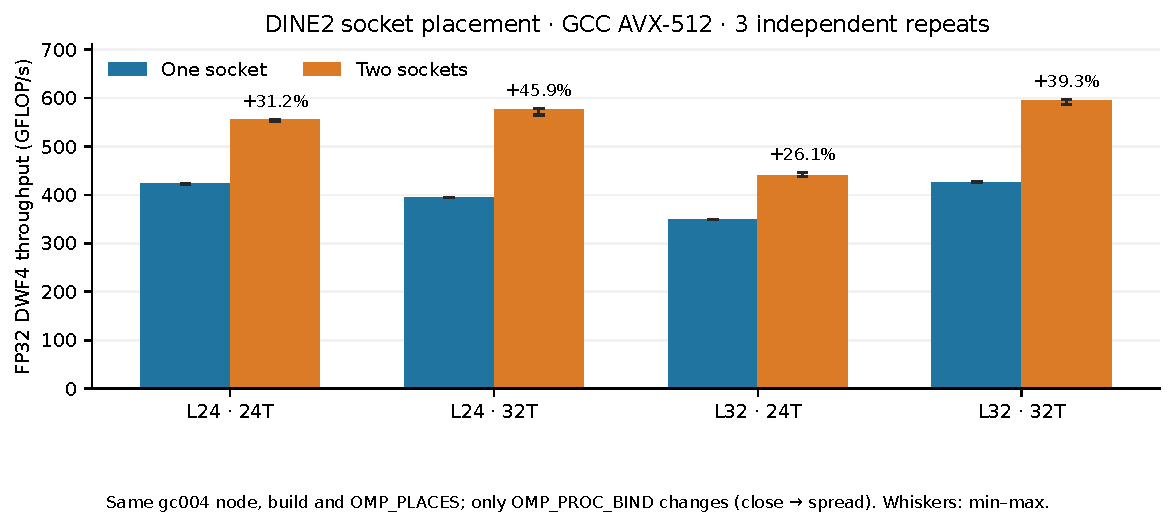
\includegraphics[width=\linewidth]{figs/dine2_socket_placement.pdf}
